\documentclass[UTF8]{ctexart}
\usepackage[a4paper,margin=2.5cm]{geometry}
\usepackage{amsmath,amssymb}
\usepackage{graphicx}
\usepackage{booktabs}
\usepackage{hyperref}
\hypersetup{hidelinks}
\usepackage{array}
\usepackage{enumitem}
\usepackage{fancyhdr}

\setmainfont{Times New Roman}
\setCJKmainfont{SimSun}
\setCJKfamilyfont{fs}{FangSong}
\newcommand{\fs}{\CJKfamily{fs}}
\newcommand{\paperfont}{\fs\fontsize{14pt}{23pt}\selectfont}
\newcommand{\checkedbox}{\ensuremath{\rlap{\raisebox{0.1ex}{\checkmark}}\square}}
\newcommand{\emptybox}{\ensuremath{\square}}
\newcommand{\examrowheight}{\rule{0pt}{27pt}}
\newcolumntype{L}[1]{>{\raggedright\arraybackslash}p{#1}}

\fancypagestyle{exampaper}{%
	\fancyhf{}%
	\renewcommand{\headrulewidth}{0pt}%
	\renewcommand{\footrulewidth}{0pt}%
	\fancyfoot[C]{\fs\fontsize{10.5pt}{12pt}\selectfont 第 \thepage 页 共 \pageref*{exam:lastpage} 页}%
}

\newcommand{\InsertExamSample}{%
	\clearpage
	\newgeometry{top=2.54cm,bottom=2.54cm,left=3.17cm,right=3.17cm,footskip=1.15cm}%
	\pagestyle{exampaper}%
	\setcounter{page}{1}%
	\begingroup
	\paperfont
	\setlength{\parindent}{0pt}%
	\setlength{\parskip}{0pt}%
	\setlength{\abovedisplayskip}{5pt}%
	\setlength{\belowdisplayskip}{5pt}%
	\setlength{\abovedisplayshortskip}{3pt}%
	\setlength{\belowdisplayshortskip}{3pt}%
	\setlist[enumerate,1]{label=\arabic*.,leftmargin=1.55em,labelsep=0.35em,itemsep=0pt,topsep=0pt,parsep=0pt,partopsep=0pt}%
	\setlist[enumerate,2]{label=(\arabic*),leftmargin=2.5em,labelsep=0.25em,itemsep=0pt,topsep=0pt,parsep=0pt,partopsep=0pt}%
	\setlist[itemize]{label=\textbullet,leftmargin=2.4em,itemsep=0pt,topsep=0pt,parsep=0pt,partopsep=0pt}%
	
	\begin{center}
		{\songti\bfseries\fontsize{16pt}{20pt}\selectfont 复旦大学研究生课程考试试卷}\\[13pt]
		{\fontsize{14pt}{18pt}\selectfont （2025  - 2026 学年第 2 学期）}
	\end{center}
	
	\vspace{8pt}
	
	{\fontsize{14pt}{17pt}\selectfont
		\setlength{\tabcolsep}{0pt}
		\renewcommand{\arraystretch}{1.02}
		\begin{center}
			\begin{tabular}{@{}L{2.45cm}L{5.55cm}L{2.45cm}L{4.15cm}@{}}
				\examrowheight 授课学期： & 春季 & 考试日期： & 2026-7-1 \\
				\examrowheight 课程名称： & 神经网络的模型与应用 & 课程代码： & MATH40054 \\
				\examrowheight 开课院系： & 数学科学学院 & 试卷类型： & \checkedbox A 卷\quad \emptybox B 卷 \\
				\examrowheight 考试形式： & \multicolumn{3}{L{12.15cm}}{\emptybox 开卷\quad \emptybox 闭卷\quad \emptybox 课程论文\quad \checkedbox 其他} \\
				\multicolumn{4}{@{}L{14.6cm}@{}}{\examrowheight 姓名：\quad 盖括\hspace{1.65cm} 学号：\quad 25110180015\hspace{1.30cm} 成绩：} \\
			\end{tabular}
		\end{center}
	}
	
	\vspace{24pt}
	
	\begin{center}
		（共7题，每题20分，选5道题完成即可）
	\end{center}
	
	\vspace{28pt}
	
	\begin{enumerate}
		\item 对于如下过程描述的LIF模型
		\[
		\frac{dV}{dt}=-g_LV+g_{\mathrm{syn}}I_{\mathrm{syn}}
		\]
		\[
		\tau\frac{dI_{\mathrm{syn}}}{dt}=-I_{\mathrm{syn}}+\mu+\sigma\frac{dW}{dt}
		\]
		这里W是一个标准的Wiener过程，膜电位达到阈值$V_{th}$产生动过电位放电，存在复位周期$\tau_{ref}$。$I_{syn}$描述（一个）突触电流，$\tau$是其时间常数。$\mu$、$\sigma$、$g_{syn}$、$\tau$、$g_L$皆为常数。对此动作电位发放点稳态过程的Inter-Spike-Interval的随机变量记为$T$：
		\par (1) 给出$T$的期望和方差的表达式，推导该神经元动作电位发放的更新函数(renewal function）的期望和方差表达式；
		\par (2) 给定任意的期望$m$和方差$\sigma^2$，如何构造参数$(g_{syn},\mu,\sigma)$（给定
		\newpage
		其他常数）,使得$T$的期望和方差分别等于或者近似$m$和$\sigma^2$，并通过数值模拟来验证你的结果。
		
		\item 对于一个ordinary renewal process（$X_1,X_2,\cdots,X_n,\cdots$），假设已知其更新间隔$X_n$各阶统计量，请推导该神经元动作电位发放的更新函数(renewal function）的n阶统计量的表达式。
		
		\item 考虑如下兴奋-抑制神经网络模型
		\[
		\tau_E\frac{dv_E}{dt}=-v_E+\left[M_{EE}v_E-M_{EI}v_I+h_E\right]^+
		\]
		\[
		\tau_I\frac{dv_I}{dt}=-v_I+\left[M_{IE}v_E-M_{II}v_I+h_I\right]^+
		\]
		$[z]^+=\max\{z,0\}$, $v_{E,I}$分别表示兴奋性/抑制性神经元群的发放率，$M_{ab}$分别是对应链接权重，a,b=E,I, $h_{E,I}$分别是兴奋性/抑制性神经元群接收到的外部刺激。分别给出该系统对应参数$\tau_I$和$h_E$的Hopf分叉分析，并给以实际数值模拟进行验证。
		
		\item 多神经元对刺激方向的响应模型如下。假设每个神经元的条件发放率表示如下
		\[
		f_a(s)=\exp\left(-\frac{(s-s_a)^2}{2\sigma_a^2}\right)
		\]
		其中a=1，…,N是神经元编号，s是受到外部刺激的方向角度（$[0,180^\circ]$），$s_a$是神经元a的偏好方向，$\sigma_a>0$是神经元调谐函数的参数。假设
		\newpage
		\par {\Large$\bullet$}\quad 神经元动作电位发放之间是统计独立的；
		\par {\Large$\bullet$}\quad 神经元动作电位发放是一个泊松过程。
		\par 假设贝叶斯损失为平方差：
		\[
		loss=(s-\hat{s})^2
		\]
		$\hat{s}$是估计方向角度。
		
		通过这N个神经元的动作电位发放时间点，建立对外部刺激方向s的最小方差的无偏(MVUB)估计，并计算其平方误差。可给出解析解，或者近似解，并进行数值模拟验证。
		
		\item 分离附件中音频数据中的源信号并评估质量，并且比较至少两种算法。
		
		\item 构建神经网络对MNIST数据集进行0-9手写数字的分类，并分别利用随机梯度下降（SGD）和自然梯度（NG）进行训练，并进行对比。
		
		\item 利用Reinforcement Learning算法求解迷宫最短路径搜索问题。\par 迷宫图请见附件(maze.jpg；黄色是出发位置)。
	\end{enumerate}
	
	要求：任意给出中点位置，规划出最短路径或者告知不能到达。最好给出交互式的界面。
	\label{exam:lastpage}%
	\endgroup
	\clearpage
	\restoregeometry
	\pagestyle{plain}%
	\setcounter{page}{1}%
	\normalfont\normalsize
}
\title{期末报告}
\author{盖括 25110180015}
\date{\today}

\begin{document}
\InsertExamSample

	\emergencystretch=2em
	\maketitle

\section{第一题}


\subsection{第（1）问}

ISI 矩与更新函数的推导：

LIF 模型为
\begin{align}
	\frac{dV}{dt} &= -g_L V + g_{\mathrm{syn}} I_{\mathrm{syn}}, \label{eq:lif_v}\\
	\tau \frac{d I_{\mathrm{syn}}}{dt}
	&= - I_{\mathrm{syn}}+\mu+\sigma \frac{dW}{dt}, \label{eq:lif_i}
\end{align}
其中 $W$ 为标准 Wiener 过程。膜电位达到阈值 $V_{\mathrm{th}}$ 时产生一次动作电位，
随后经历绝对不应期 $\tau_{\mathrm{ref}}$。题目未给出重置电位，本文取
$V_{\mathrm{r}}=0$。连续两次发放之间的间隔记为
\[
T=\tau_{\mathrm{ref}}+\tau_h,
\]
其中 $\tau_h$ 是从重置电位 $V_{\mathrm r}$ 首次到达阈值 $V_{\mathrm{th}}$ 的首达时间。
若每次发放后系统按同一规则重置，则 $T_1,T_2,\ldots$ 可看作独立同分布的更新间隔，
从而放电计数过程
\[
N(t)=\max\{n:S_n\le t\},\qquad S_n=T_1+\cdots+T_n
\]
构成普通更新过程。




由式 \eqref{eq:lif_i} 可写成
\[
dI_{\mathrm{syn}}
=\frac{\mu-I_{\mathrm{syn}}}{\tau}\,dt+\frac{\sigma}{\tau}\,dW_t.
\]
这是均值为 $\mu$ 的 OU 过程，其稳态协方差为
\[
\operatorname{Cov}\bigl(I_{\mathrm{syn}}(t),I_{\mathrm{syn}}(t+s)\bigr)
=\frac{\sigma^2}{2\tau}e^{-|s|/\tau}.
\]
当突触相关时间 $\tau$ 相对放电时间尺度较小时，有
\[
\operatorname{Var}\left(\int_0^t (I_{\mathrm{syn}}(s)-\mu)\,ds\right)
\approx t\cdot 2\int_0^\infty \frac{\sigma^2}{2\tau}e^{-s/\tau}\,ds
=\sigma^2 t.
\]
因此可用有效一维扩散近似
\begin{equation}
	dV_t=(-g_LV_t+A)\,dt+B\,dB_t,\qquad
	A=g_{\mathrm{syn}}\mu,\quad B=g_{\mathrm{syn}}\sigma,
	\label{eq:effective_diffusion}
\end{equation}
来描述膜电位的首达时间。这里 $B_t$ 是另一个标准布朗运动。

下面计算首达时间的一阶矩和二阶矩：

对扩散过程 \eqref{eq:effective_diffusion}，其生成元为
\[
\mathcal L f(x)=(-g_Lx+A)f'(x)+\frac{B^2}{2}f''(x).
\]
设
\[
u_n(x)=\mathbb E_x[\tau_h^n],\qquad u_0(x)=1.
\]
由 Dynkin 公式或后向 Kolmogorov 方程，首达时间矩满足递推边值问题
\begin{equation}
	\mathcal L u_n(x)=-n u_{n-1}(x),\qquad x<V_{\mathrm{th}},
	\label{eq:moment_ode}
\end{equation}
并具有边界条件
\[
u_n(V_{\mathrm{th}})=0,\qquad u_n(x)\text{ 在 }x\to-\infty\text{ 时有界}.
\]
具体地，一阶矩满足
\begin{equation}
	(-g_Lx+A)u_1'(x)+\frac{B^2}{2}u_1''(x)=-1,
	\qquad u_1(V_{\mathrm{th}})=0,
	\label{eq:first_moment_ode}
\end{equation}
二阶矩满足
\begin{equation}
	(-g_Lx+A)u_2'(x)+\frac{B^2}{2}u_2''(x)=-2u_1(x),
	\qquad u_2(V_{\mathrm{th}})=0.
	\label{eq:second_moment_ode}
\end{equation}
令
\[
\Phi(x)=\int^x \frac{2(-g_Ly+A)}{B^2}\,dy
=\frac{2Ax-g_Lx^2}{B^2}.
\]
将 \eqref{eq:moment_ode} 视为关于 $u_n'(x)$ 的一阶线性方程，可得递推积分表达式
\begin{equation}
	u_n(x)=
	n\int_x^{V_{\mathrm{th}}}
	e^{-\Phi(y)}
	\int_{-\infty}^{y}\frac{2}{B^2}e^{\Phi(z)}u_{n-1}(z)\,dz\,dy .
	\label{eq:moment_integral}
\end{equation}
于是 ISI 的均值和方差为
\begin{align}
	\mathbb E[T]
	&=\tau_{\mathrm{ref}}+u_1(V_{\mathrm r}), \label{eq:isi_mean}\\
	\operatorname{Var}(T)
	&=u_2(V_{\mathrm r})-u_1(V_{\mathrm r})^2. \label{eq:isi_var}
\end{align}
其中不应期是确定常数，因此只改变均值，不改变方差。


记 $F(t)=\mathbb P(T\le t)$，$F^{*n}$ 为 $F$ 的 $n$ 重卷积。由于
\[
N(t)\ge n \iff S_n=T_1+\cdots+T_n\le t,
\]
有
\[
\mathbb P(N(t)\ge n)=F^{*n}(t).
\]
利用非负整数随机变量恒等式
\[
N(t)=\sum_{n=1}^{\infty}\mathbf 1_{\{N(t)\ge n\}},
\]
两边取期望得到更新函数
\begin{equation}
	M(t)=\mathbb E[N(t)]
	=\sum_{n=1}^{\infty}F^{*n}(t).
	\label{eq:renewal_mean_exact}
\end{equation}
若 $\widehat F(s)$ 表示 $F$ 的 Laplace--Stieltjes 变换，则
\[
\mathcal L\{F^{*n}\}(s)=\frac{\widehat F(s)^n}{s},
\]
因此
\begin{equation}
	\widehat M(s)
	=\frac{1}{s}\sum_{n=1}^{\infty}\widehat F(s)^n
	=\frac{\widehat F(s)}{s(1-\widehat F(s))}.
	\label{eq:renewal_laplace}
\end{equation}


同样利用整数变量恒等式
\[
N(t)^2=\sum_{n=1}^{N(t)}(2n-1)
=\sum_{n=1}^{\infty}(2n-1)\mathbf 1_{\{N(t)\ge n\}},
\]
取期望得
\begin{equation}
	\mathbb E[N(t)^2]
	=\sum_{n=1}^{\infty}(2n-1)F^{*n}(t).
	\label{eq:renewal_second_exact}
\end{equation}
从而
\begin{equation}
	\operatorname{Var}(N(t))
	=\sum_{n=1}^{\infty}(2n-1)F^{*n}(t)-M(t)^2.
	\label{eq:renewal_var_exact}
\end{equation}
其二阶矩的 Laplace 形式为
\begin{equation}
	\mathcal L\{\mathbb E[N(t)^2]\}(s)
	=\frac{1}{s}\sum_{n=1}^{\infty}(2n-1)\widehat F(s)^n
	=\frac{\widehat F(s)(1+\widehat F(s))}
	{s(1-\widehat F(s))^2}.
	\label{eq:renewal_second_laplace}
\end{equation}
若只关心长时间近似，并令
\[
m_T=\mathbb E[T],\qquad v_T=\operatorname{Var}(T),
\]
则普通更新定理和更新中心极限定理给出
\begin{equation}
	\mathbb E[N(t)]\sim \frac{t}{m_T},
	\qquad
	\operatorname{Var}(N(t))\sim \frac{v_T}{m_T^3}\,t,
	\qquad t\to\infty.
	\label{eq:renewal_asymptotic}
\end{equation}
这说明平均放电率为 $1/m_T$，而计数方差的增长率由 ISI 方差 $v_T$ 决定。

\subsection{第（2）问}

给定目标
\[
\mathbb E[T]\approx m,\qquad \operatorname{Var}(T)\approx s^2,
\]
由 \eqref{eq:isi_mean}--\eqref{eq:isi_var} 可知，只需要调节有效漂移 $A$ 和有效扩散强度
$B$。因为
\[
A=g_{\mathrm{syn}}\mu,\qquad B=g_{\mathrm{syn}}\sigma,
\]
三元组 $(g_{\mathrm{syn}},\mu,\sigma)$ 并不唯一。本文取 $g_{\mathrm{syn}}=1$，
然后令
\[
\mu=A,\qquad \sigma=B.
\]
若希望固定其他正值 $g_{\mathrm{syn}}=c$，则只需取
\[
\mu=\frac{A}{c},\qquad \sigma=\frac{B}{c}.
\]

具体构造步骤如下。

\begin{enumerate}
	\item 先扣除不应期，令目标首达时间均值为
	\[
	\bar m=m-\tau_{\mathrm{ref}}.
	\]
	必须有 $\bar m>0$。
	\item 对给定 $B$，用有限差分求解 \eqref{eq:first_moment_ode}--\eqref{eq:second_moment_ode}。
	边界上取 $u_n(V_{\mathrm{th}})=0$，左端取足够远的反射边界近似自然边界。
	\item 对给定 $B$，用二分法寻找 $A$，使
	\[
	u_1(V_{\mathrm r};A,B)=\bar m.
	\]
	\item 再对 $B$ 做二分法，使
	\[
	u_2(V_{\mathrm r};A,B)-u_1(V_{\mathrm r};A,B)^2=s^2.
	\]
	\item 得到 $A,B$ 后构造
	\[
	(g_{\mathrm{syn}},\mu,\sigma)=\left(1,A,B\right).
	\]
\end{enumerate}

这里还需要说明一个数值边界处理。理论推导中，后向方程的左边界条件写为
$x\to-\infty$ 时 $u_n(x)$ 有界，这对应扩散过程在远离阈值的左侧没有吸收边界。
但在 Python 中不能在无穷区间上直接求解有限差分方程，因此代码把计算区间截断为
\[
[x_{\min},V_{\mathrm{th}}],
\qquad
x_{\min}
=\min\left\{
V_{\mathrm r}-7\frac{B}{\sqrt{2g_L}}-1,\,-2
\right\}.
\]
其中 $B/\sqrt{2g_L}$ 是有效 OU 型膜电位扩散的稳态标准差尺度。这样选取
$x_{\min}$ 可以保证左边界远低于重置电位和主要概率质量区域。数值上在
$x_{\min}$ 处使用反射边界
\[
u_n(x_0)-u_n(x_1)=0,
\]
也就是近似令 $u_n'(x_{\min})=0$。这不是改变理论模型，而是用一个足够远的有限边界
近似理论中的自然边界条件；当 $x_{\min}$ 继续向左移动时，该截断误差会迅速减小。

数值搜索的初值可由无噪声确定性 LIF 给出。若 $B=0$，膜电位轨道为
\[
V(t)=\frac{A}{g_L}+\left(V_{\mathrm r}-\frac{A}{g_L}\right)e^{-g_Lt}.
\]
令 $V(\bar m)=V_{\mathrm{th}}$，得到
\[
A_0=
\frac{g_L\left(V_{\mathrm{th}}-V_{\mathrm r}e^{-g_L\bar m}\right)}
{1-e^{-g_L\bar m}}.
\]
这给出了漂移大小的合理初始范围；随后用后向方程精确匹配目标矩。

\textbf{Python 数值模拟:}

模拟使用原始二维模型
\begin{align*}
	dI_{\mathrm{syn}}
	&=\frac{\mu-I_{\mathrm{syn}}}{\tau}\,dt+\frac{\sigma}{\tau}\,dW_t,\\
	dV_t&=(-g_LV_t+g_{\mathrm{syn}}I_{\mathrm{syn}})\,dt,
\end{align*}
而不是只模拟一维扩散近似。每个 ISI 从 $V_{\mathrm r}=0$ 开始，$I_{\mathrm{syn}}(0)$
从 OU 稳态分布
\[
I_{\mathrm{syn}}(0)\sim \mathcal N\left(\mu,\frac{\sigma^2}{2\tau}\right)
\]
抽样，用 Euler--Maruyama 格式推进；到达阈值后用线性插值估计穿越时间，并加上
$\tau_{\mathrm{ref}}$ 得到完整 ISI。

代码中默认目标和常数为
\[
m=1.0,\qquad s^2=0.08,\qquad
g_L=0.2,\quad \tau=0.02,\quad
V_{\mathrm r}=0,\quad V_{\mathrm{th}}=1,\quad \tau_{\mathrm{ref}}=0.05.
\]


程序构造出的参数为
\begin{center}
	\begin{tabular}{ll}
		\toprule
		参数 & 数值 \\
		\midrule
		$g_{\mathrm{syn}}$ & $1.000000$ \\
		$\mu$ & $1.146884$ \\
		$\sigma$ & $0.306647$ \\
		$A=g_{\mathrm{syn}}\mu$ & $1.146884$ \\
		$B=g_{\mathrm{syn}}\sigma$ & $0.306647$ \\
		\bottomrule
	\end{tabular}
\end{center}

理论构造与原始模型仿真对比如下：
\begin{center}
	\begin{tabular}{lcc}
		\toprule
		来源 & $\mathbb E[T]$ & $\operatorname{Var}(T)$ \\
		\midrule
		目标值 & $1.000000$ & $0.080000$ \\
		扩散近似后向方程 & $1.000000$ & $0.080000$ \\
		原始二维 SDE 仿真 & $1.032638$ & $0.079216$ \\
		\bottomrule
	\end{tabular}
\end{center}
仿真使用 $8000$ 个独立 ISI，时间步长为 $5\times 10^{-4}$。相对误差为
\[
\frac{\widehat{\mathbb E[T]}-m}{m}=3.26\%,\qquad
\frac{\widehat{\operatorname{Var}(T)}-s^2}{s^2}=-0.98\%.
\]
均值有小幅偏大，主要来自三类误差。第一，参数构造基于短相关时间极限下的一维有效扩散近似，
而验证时使用的是带有限相关时间 $\tau=0.02$ 的原始 OU 突触电流。更具体地，
\[
\operatorname{Var}\left(\int_0^t(I_{\mathrm{syn}}(s)-\mu)\,ds\right)
=\sigma^2\left[t-\tau\left(1-e^{-t/\tau}\right)\right],
\]
只有在 $\tau\to0$ 或 $t\gg \tau$ 的极限下才收敛到有效扩散模型使用的
$\sigma^2t$。因此随着 $\tau\to0$，原始二维模型会更接近一维扩散近似，均值误差也应进一步收敛。
第二，阈值穿越由 Euler--Maruyama 离散步长 $dt=5\times10^{-4}$ 和线性插值近似，
仍会留下小的离散化误差。第三，Monte Carlo 样本量有限；本次 $8000$ 个 ISI 下，
均值标准误约为 $\sqrt{0.079216/8000}\approx0.0031$，明显小于 $3.26\%$ 的系统偏差，
说明有限相关时间近似是主要来源，而方差的 $-0.98\%$ 偏差已在采样波动量级内。
总体上，构造参数能较好地达到给定 ISI 方差，并使均值保持在目标附近。

\begin{figure}[htbp]
	\centering
	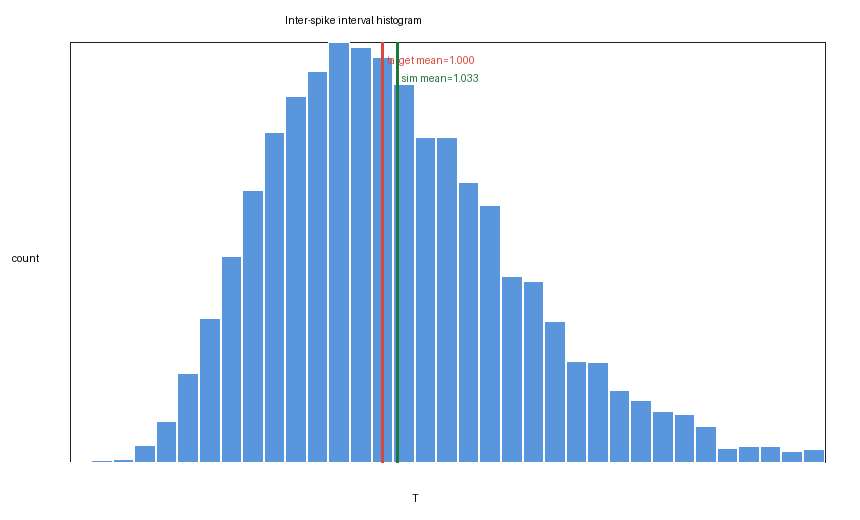
\includegraphics[width=0.82\linewidth]{results/isi_histogram.png}
	\caption{模拟得到的 ISI 分布直方图}
	\label{fig:isi_hist}
\end{figure}

图 \ref{fig:isi_hist} 给出了 $8000$ 个 ISI 样本的直方图。红色竖线是目标均值
$m=1.0$，绿色竖线是原始二维 SDE 仿真得到的样本均值 $1.032638$。两条竖线接近，
说明参数构造达到了题目要求的“等于或者近似”目标。直方图略向右偏，这是首达时间分布的典型形态：
大多数轨道在平均时间附近穿越阈值，但少数受到负向噪声影响的轨道会显著延迟。

\begin{figure}[htbp]
	\centering
	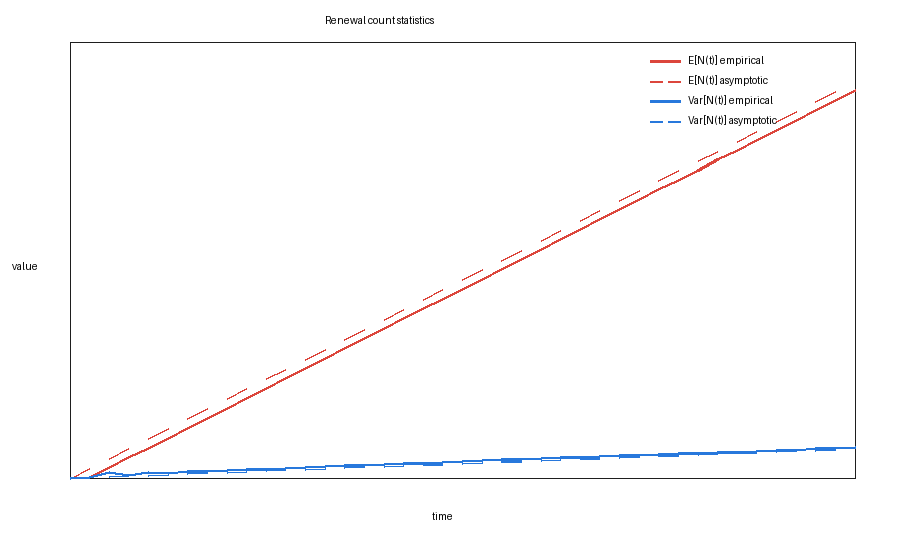
\includegraphics[width=0.86\linewidth]{results/renewal_counts.png}
	\caption{更新计数 $N(t)$ 的经验均值、方差与渐近公式对比}
	\label{fig:renewal_counts}
\end{figure}

图 \ref{fig:renewal_counts} 用模拟得到的 ISI 样本重抽样生成多个更新过程，计算不同时间 $t$
下 $N(t)$ 的经验均值与经验方差。红色实线为经验 $\mathbb E[N(t)]$，红色虚线为
$t/\widehat m_T$；蓝色实线为经验 $\operatorname{Var}(N(t))$，蓝色虚线为
$\widehat v_Tt/\widehat m_T^3$。可以看到，随着时间增大，经验均值和方差都沿着更新理论给出的
渐近直线增长，验证了第（1）问中的更新函数推导。



总体而言，第（1）问中，ISI 可表示为确定不应期加扩散过程首达时间，其矩由后向 Kolmogorov 方程
\eqref{eq:moment_ode} 递推给出；更新计数的均值和方差则由 $F^{*n}$ 的卷积级数给出，
长时间下满足 $\mathbb E[N(t)]\sim t/m_T$ 与
$\operatorname{Var}(N(t))\sim v_Tt/m_T^3$。第（2）问中，利用
$A=g_{\mathrm{syn}}\mu$、$B=g_{\mathrm{syn}}\sigma$ 的非唯一性，可先求有效参数
$A,B$，再构造 $(g_{\mathrm{syn}},\mu,\sigma)$。数值模拟表明，在默认目标
$m=1.0,s^2=0.08$ 下，构造参数使原始模型的 ISI 均值和方差与目标值较为接近。






\section{第二题}

对于神经元动作电位发放，假设连续两次发放的时间间隔 $X_1, X_2, \cdots, X_n, \cdots$ 独立同分布，构成一个普通更新过程 。
设 $X_i$ 的概率密度函数为 $f(t)$，累积分布函数为 $F(t)$。设在 $(0, t]$ 时间内的发放总数（更新次数）为 $N(t)$。

更新过程 $N(t)$ 的 $n$ 阶矩记为 $m_n(t) = E[N(t)^n]$。。

已知 $X_n$ 的各阶统计量，即原点矩 $\mu_k = E[X^k]$，这等价于已知 $X_n$ 的拉普拉斯变换展开。下面通过拉普拉斯变换域和时间域两种方法推导 $m_n(t)$ 的表达式。

利用拉普拉斯变换与概率生成函数：

事件 $N(t) \ge k$ 等价于第 $k$ 次更新的时间 $S_k \le t$。设 $F_k(t)$ 为 $f(t)$ 的 $k$ 重卷积，可知 $N(t)$ 的概率分布为：
\begin{equation}
	P(N(t) = k) = F_k(t) - F_{k+1}(t) \quad (F_0(t) \equiv 1)
\end{equation}

定义 $N(t)$ 的概率生成函数 为 $G(z, t)$：
\begin{equation}
	G(z, t) = E[z^{N(t)}] = \sum_{k=0}^{\infty} z^k (F_k(t) - F_{k+1}(t)) = 1 + (z-1) \sum_{k=1}^{\infty} z^{k-1} F_k(t)
\end{equation}

对 $t$ 取拉普拉斯变换 $\mathcal{L}\{\cdot\}$。已知 $\mathcal{L}\{F_k(t)\} = \frac{1}{s} [\tilde{f}(s)]^k$，其中 $\tilde{f}(s)$ 是 $f(t)$ 的拉普拉斯变换，由已知的各阶矩 $\mu_k$ 可展开为 $\tilde{f}(s) = \sum_{j=0}^{\infty} \frac{(-1)^j}{j!} \mu_j s^j$。对生成函数取拉普拉斯变换得：
\begin{equation}
	\hat{G}(z, s) = \frac{1}{s} + \frac{z-1}{s} \sum_{k=1}^{\infty} z^{k-1} [\tilde{f}(s)]^k = \frac{1 - \tilde{f}(s)}{s(1 - z \tilde{f}(s))}
\end{equation}

$N(t)$ 的 $n$ 阶阶乘矩记为 $m_{(n)}(t) = E[N(t)(N(t)-1)\cdots(N(t)-n+1)]$。其拉普拉斯变换可通过求 $z$ 的 $n$ 阶偏导并在 $z=1$ 处取值获得：
\begin{equation}
	\mathcal{L}\{m_{(n)}(t)\} = \left. \frac{\partial^n}{\partial z^n} \hat{G}(z, s) \right|_{z=1} = \frac{1 - \tilde{f}(s)}{s} \frac{n! [\tilde{f}(s)]^n}{(1 - \tilde{f}(s))^{n+1}} = \frac{n! [\tilde{f}(s)]^n}{s(1 - \tilde{f}(s))^n}
\end{equation}

普通的 $n$ 阶矩 $m_n(t)$ 可以利用第二类string数 $S(n, k)$ 由阶乘矩组合得到：$N^n = \sum_{k=1}^{n} S(n, k) N(N-1)\cdots(N-k+1)$。两边取期望并进行拉普拉斯变换，最终得到 $n$ 阶统计量在 $s$ 域的表达式：
\begin{equation}
	\hat{m}_n(s) = \sum_{k=1}^{n} S(n, k) \frac{k! [\tilde{f}(s)]^k}{s(1 - \tilde{f}(s))^k}
\end{equation}

\textbf{另一个角度是利用全概率公式与更新方程：}

考虑首次动作电位发放的时间 $X_1 = x$。若 $x > t$，则 $N(t) = 0$；若 $x \le t$，则 $N(t) = 1 + N(t-x)$。根据全概率公式有：
\begin{equation}
	m_n(t) = E[N(t)^n] = \int_0^t E[(1 + N(t-x))^n] dF(x)
\end{equation}

利用二项式定理展开 $(1 + N(t-x))^n$：
\begin{equation}
	m_n(t) = \int_0^t \sum_{k=0}^{n} \binom{n}{k} m_k(t-x) dF(x)
\end{equation}

提出 $k=0$ 和 $k=n$ 的项，并写成卷积形式：
\begin{equation}
	m_n(t) = F(t) + \sum_{k=1}^{n-1} \binom{n}{k} (m_k * f)(t) + (m_n * f)(t)
\end{equation}

移项得标准更新方程 $m_n(t) - (m_n * f)(t) = h_n(t)$，其中已知驱动项为 $h_n(t) = F(t) + \sum_{k=1}^{n-1} \binom{n}{k} (m_k * f)(t)$。根据更新方程定理，其解为：
\begin{equation}
	m_n(t) = h_n(t) + \int_0^t h_n(t-x) dM(x)
\end{equation}
此处 $M(t) = m_1(t)$ 为一阶更新函数。该式给出了时间域下 $n$ 阶统计量的递推表达式。


\section{第三题}
\subsection{兴奋-抑制神经网络的 Hopf 分叉分析}

兴奋-抑制神经网络模型：
\begin{align}
	\tau_E\frac{dv_E}{dt}
	&=-v_E+\bigl[M_{EE}v_E-M_{EI}v_I+h_E\bigr]_+,
	\label{eq:model_e}\\
	\tau_I\frac{dv_I}{dt}
	&=-v_I+\bigl[M_{IE}v_E-M_{II}v_I+h_I\bigr]_+,
	\label{eq:model_i}
\end{align}
其中
\[
[z]_+=\max\{z,0\}.
\]
$v_E,v_I$ 分别表示兴奋性和抑制性神经元群发放率，$M_{ab}$ 为连接权重，
$h_E,h_I$ 为外部输入。

由于模型使用 ReLU 非线性，它是分段线性系统。在任意一个固定活动区中，右端关于
$(v_E,v_I)$ 是线性的；当平衡点落在双活动区，即两个 ReLU 括号内都为正时，可以进行
通常的局部线性化分析。若平衡点穿越 ReLU 的折点边界，则发生的是非光滑的边界切换，
不属于经典光滑 Hopf 分叉。

\textbf{双活动区中的平衡点：}

在双活动区中有
\[
M_{EE}v_E-M_{EI}v_I+h_E>0,\qquad
M_{IE}v_E-M_{II}v_I+h_I>0.
\]
此时模型化为线性仿射系统
\begin{align}
	\tau_E\dot v_E
	&=(M_{EE}-1)v_E-M_{EI}v_I+h_E,\\
	\tau_I\dot v_I
	&=M_{IE}v_E-(M_{II}+1)v_I+h_I.
\end{align}
令
\[
a=M_{EE}-1,\qquad b=-M_{EI},\qquad
c=M_{IE},\qquad d=-(M_{II}+1).
\]
平衡点满足
\[
\begin{pmatrix}
	a & b\\
	c & d
\end{pmatrix}
\begin{pmatrix}
	v_E^*\\v_I^*
\end{pmatrix}
=
\begin{pmatrix}
	-h_E\\-h_I
\end{pmatrix}.
\]
矩阵行列式为
\[
K=ad-bc=M_{EI}M_{IE}-(M_{EE}-1)(M_{II}+1).
\]
若 $K\ne0$，则双活动区候选平衡点为
\begin{align}
	v_E^*
	&=\frac{(M_{II}+1)h_E-M_{EI}h_I}{K},
	\label{eq:eq_ve}\\
	v_I^*
	&=\frac{M_{IE}h_E-(M_{EE}-1)h_I}{K}.
	\label{eq:eq_vi}
\end{align}
该平衡点真正属于双活动区，需要
\[
v_E^*>0,\qquad v_I^*>0.
\]
在 $K>0$ 且 $h_I>0$ 的常见情形下，这等价于
\begin{equation}
	h_E>
	\max\left\{
	\frac{M_{EI}h_I}{M_{II}+1},
	\frac{(M_{EE}-1)h_I}{M_{IE}}
	\right\}.
	\label{eq:active_boundary}
\end{equation}

\textbf{参数 $\tau_I$ 的 Hopf 分叉分析：}

在双活动区中，系统在平衡点处的雅可比矩阵为
\begin{equation}
	J=
	\begin{pmatrix}
		\dfrac{M_{EE}-1}{\tau_E} & -\dfrac{M_{EI}}{\tau_E}\\[8pt]
		\dfrac{M_{IE}}{\tau_I} & -\dfrac{M_{II}+1}{\tau_I}
	\end{pmatrix}.
	\label{eq:jacobian}
\end{equation}
记迹和行列式分别为
\begin{align}
	T(\tau_I)
	&=\operatorname{tr}J
	=\frac{M_{EE}-1}{\tau_E}-\frac{M_{II}+1}{\tau_I},
	\label{eq:trace}\\
	D(\tau_I)
	&=\det J
	=\frac{M_{EI}M_{IE}-(M_{EE}-1)(M_{II}+1)}
	{\tau_E\tau_I}
	=\frac{K}{\tau_E\tau_I}.
	\label{eq:det}
\end{align}
二维系统发生 Hopf 分叉的线性条件为
\[
T(\tau_I^H)=0,\qquad D(\tau_I^H)>0,
\]
并且特征值实部要横截穿过虚轴。由 \eqref{eq:trace} 得
\begin{equation}
	\tau_I^H
	=\tau_E\frac{M_{II}+1}{M_{EE}-1}.
	\label{eq:tau_hopf}
\end{equation}
因此需要
\[
M_{EE}>1,\qquad K>0.
\]
此时 Hopf 点处的特征值为
\[
\lambda_{1,2}=\pm i\omega_H,\qquad
\omega_H=\sqrt{D(\tau_I^H)}
=\sqrt{\frac{K}{\tau_E\tau_I^H}}.
\]
横截条件为
\[
\frac{dT}{d\tau_I}
=\frac{M_{II}+1}{\tau_I^2}>0,
\]
所以当 $\tau_I$ 增大并穿过 $\tau_I^H$ 时，特征值实部由负变正，平衡点由稳定焦点变为
不稳定焦点。

需要注意的是，给定模型是精确分段线性的 ReLU 系统。在平衡点附近且仍处于双活动区时，
非线性高阶项为零，因此严格的光滑 Hopf 正规形一阶 Lyapunov 系数退化。数值中观察到的
稳定振荡不是由局部三次项饱和产生，而是轨道离开双活动线性区后受到 ReLU 边界的非光滑
限制而形成。因此本文将其称为 ReLU 分段线性系统中的 Hopf 型失稳和边界饱和振荡。

\textbf{参数 $h_E$ 的 Hopf 分叉分析：}

由 \eqref{eq:eq_ve}--\eqref{eq:eq_vi} 可知，$h_E$ 会改变平衡点位置；但是由
\eqref{eq:jacobian}--\eqref{eq:det} 可知，在固定活动区内雅可比矩阵、迹和行列式都不含
$h_E$。因此，在双活动区内部改变 $h_E$ 时，
\[
\frac{\partial T}{\partial h_E}=0,\qquad
\frac{\partial D}{\partial h_E}=0,
\]
特征值不会随 $h_E$ 移动，也就不可能通过 $h_E$ 产生经典 Hopf 分叉。

$h_E$ 的作用是移动平衡点，并可能使平衡点穿过 ReLU 活动边界 \eqref{eq:active_boundary}。
这种现象是非光滑边界切换或边界碰撞，而不是 Hopf 分叉。若把 ReLU 换成光滑 Sigmoid
或光滑化 ReLU，则 $h_E$ 会改变平衡点所在位置处的增益，从而可能间接影响雅可比矩阵；
但对题目给出的精确 $[z]_+$ 模型，$h_E$ 在同一线性区中不触发 Hopf。


\subsection{数值模拟}
\textbf{数值模拟方法:}

数值积分使用四阶 Runge--Kutta 方法。为了清楚验证
理论结论，取参数
\[
\tau_E=1,\quad M_{EE}=2,\quad M_{EI}=1.5,\quad
M_{IE}=2,\quad M_{II}=1,\quad h_E=0.25,\quad h_I=0.20.
\]
此时
\[
K=1,\qquad
\tau_I^H=2,\qquad
\omega_H=\sqrt{\frac{1}{2}}\approx0.7071.
\]
平衡点为
\[
(v_E^*,v_I^*)=(0.2,0.3),
\]
并且满足双活动区条件。对 $h_E$ 而言，双活动区边界为
\[
h_E>\max\left\{\frac{1.5\times0.2}{2},\frac{1\times0.2}{2}\right\}=0.15.
\]


程序输出 $\tau_I$ 扫描、$h_E$ 扫描、时间序列和相图。扫描中振幅定义为去掉前
$55\%$ 暂态后 $v_E$ 的最大值减最小值。

\textbf{数值结果与解释}

\textbf{$\tau_I$ 扫描：}

\begin{figure}[htbp]
	\centering
	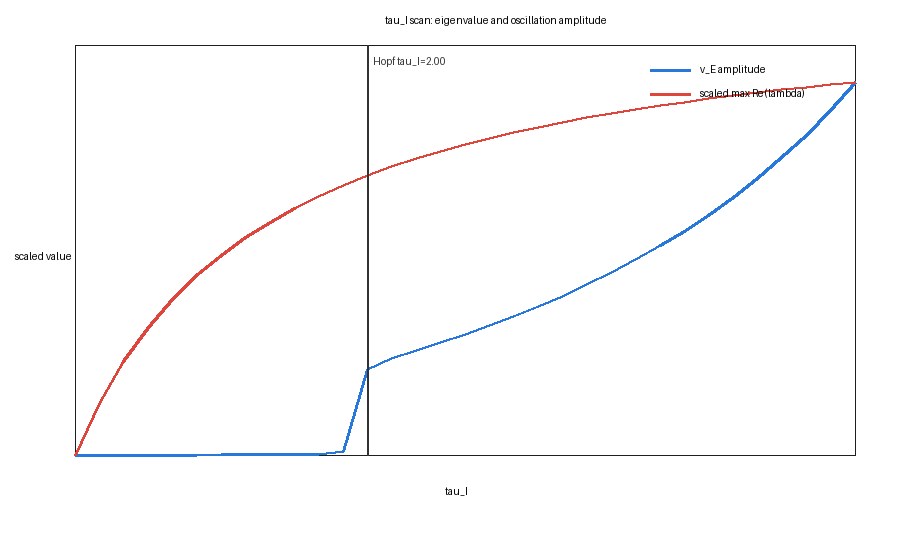
\includegraphics[width=0.86\linewidth]{results/tau_i_scan.png}
	\caption{$\tau_I$ 扫描：特征值实部穿越与振荡振幅}
	\label{fig:tau_scan}
\end{figure}

图 \ref{fig:tau_scan} 中黑色竖线为理论 Hopf 点 $\tau_I^H=2$。红线为缩放后的最大特征值实部，
蓝线为数值积分得到的 $v_E$ 振荡振幅。可以看到，当 $\tau_I<2$ 时，特征值实部为负，
轨道收敛到平衡点，振幅近似为零；当 $\tau_I>2$ 后，特征值实部为正，平衡点失稳，
轨道进入由 ReLU 边界限制的持续振荡。数值结果与 \eqref{eq:tau_hopf} 的理论临界值一致。

\begin{figure}[htbp]
	\centering
	\begin{minipage}{0.48\linewidth}
		\centering
		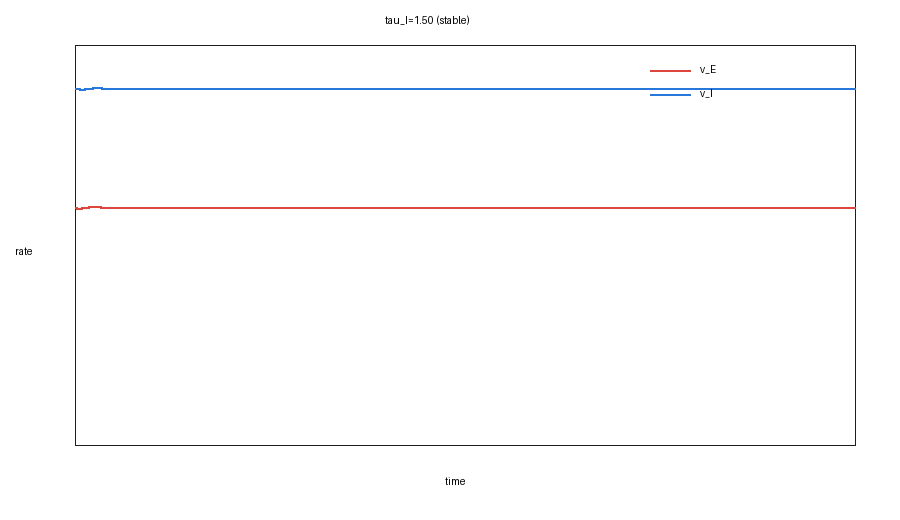
\includegraphics[width=\linewidth]{results/time_series_tau_stable.png}
		\caption{$\tau_I=1.5$ 时的稳定时间序列}
		\label{fig:stable_ts}
	\end{minipage}
	\hfill
	\begin{minipage}{0.48\linewidth}
		\centering
		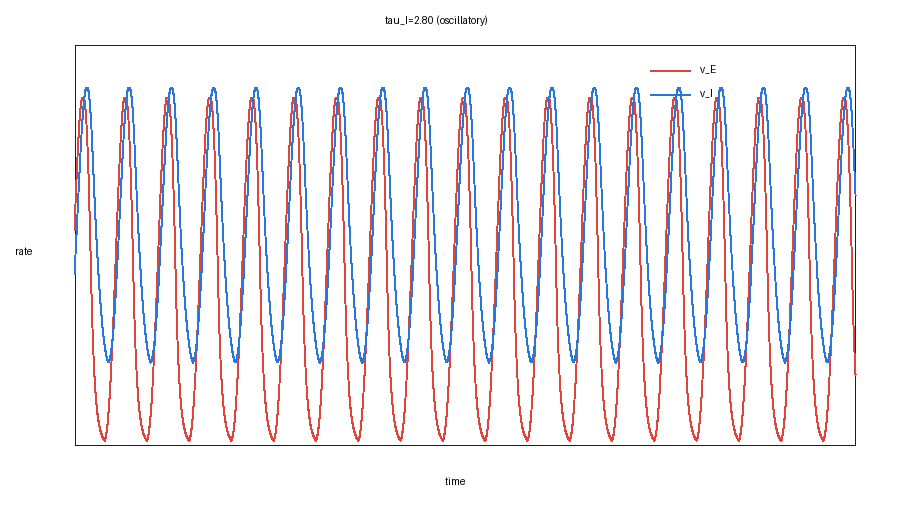
\includegraphics[width=\linewidth]{results/time_series_tau_oscillatory.png}
		\caption{$\tau_I=2.8$ 时的振荡时间序列}
		\label{fig:osc_ts}
	\end{minipage}
\end{figure}

图 \ref{fig:stable_ts} 和图 \ref{fig:osc_ts} 更直接展示了分叉前后的动力学差异。
$\tau_I=1.5$ 时，
\[
T=1-\frac{2}{1.5}=-\frac13<0,
\]
平衡点是稳定焦点，兴奋性和抑制性发放率最终趋于常数。$\tau_I=2.8$ 时，
\[
T=1-\frac{2}{2.8}>0,
\]
平衡点失稳，兴奋群和抑制群交替升降，形成稳定周期振荡。抑制群相对兴奋群有相位滞后，
这符合 E-I 反馈环中兴奋驱动抑制、抑制再压低兴奋的机制。

\begin{figure}[htbp]
	\centering
	\begin{minipage}{0.48\linewidth}
		\centering
		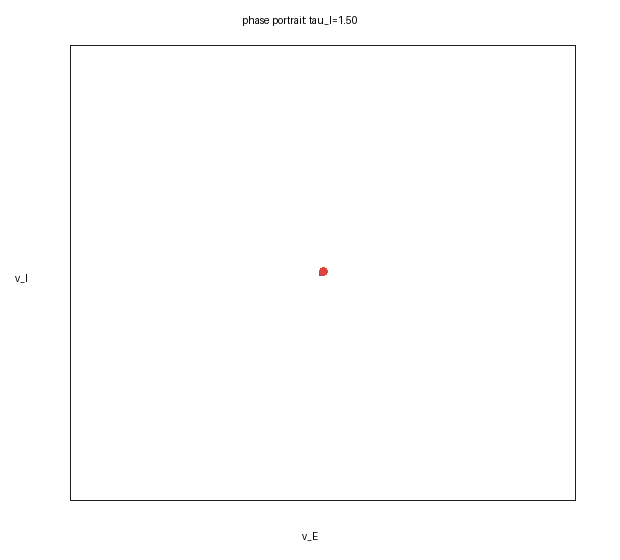
\includegraphics[width=\linewidth]{results/phase_tau_stable.png}
		\caption{$\tau_I=1.5$ 的相图}
		\label{fig:stable_phase}
	\end{minipage}
	\hfill
	\begin{minipage}{0.48\linewidth}
		\centering
		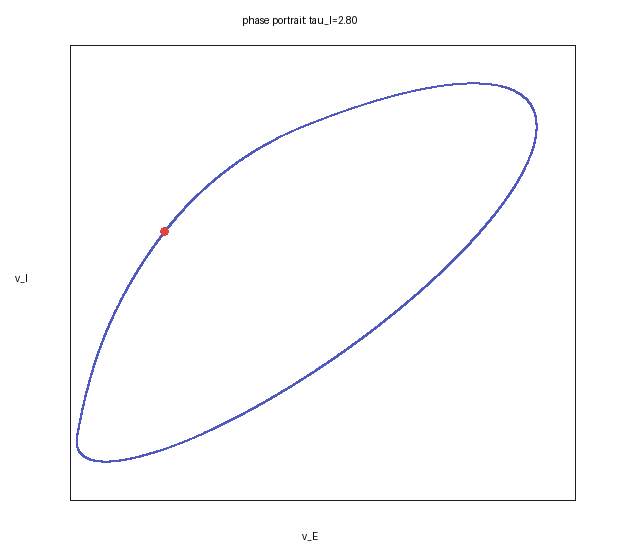
\includegraphics[width=\linewidth]{results/phase_tau_oscillatory.png}
		\caption{$\tau_I=2.8$ 的相图}
		\label{fig:osc_phase}
	\end{minipage}
\end{figure}

相图进一步说明：分叉前轨道螺旋收敛到平衡点；分叉后轨道围绕平衡点运动，并在 ReLU
分段边界作用下形成闭合环。由于模型是分段线性的，闭合环的幅值不是由局部三阶非线性决定，
而是由全局分段结构决定。

\textbf{$h_E$ 扫描：}

\begin{figure}[htbp]
	\centering
	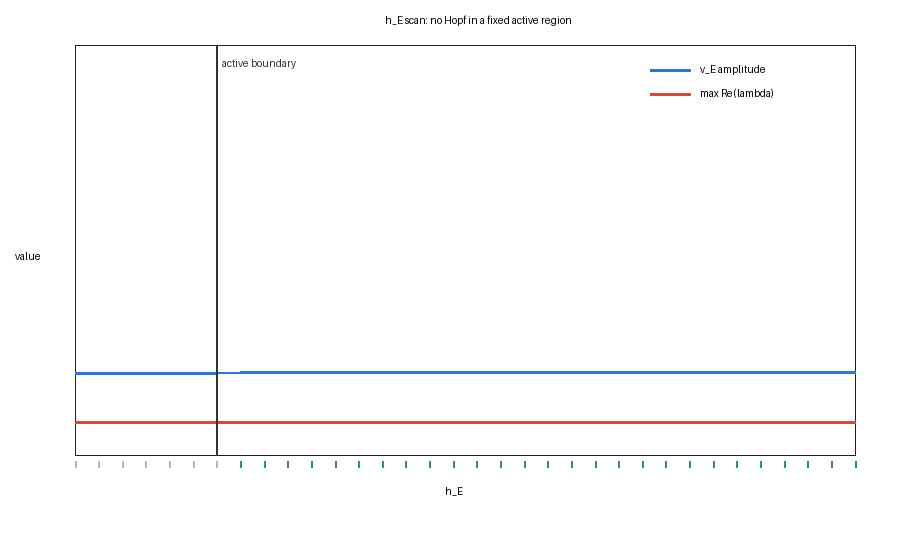
\includegraphics[width=0.86\linewidth]{results/h_e_scan.png}
	\caption{$h_E$ 扫描：固定活动区内无 Hopf 分叉}
	\label{fig:h_scan}
\end{figure}

图 \ref{fig:h_scan} 固定 $\tau_I=1.5$，扫描 $h_E$。黑色竖线是双活动区边界
$h_E=0.15$；底部绿色短线表示候选平衡点位于双活动区。红线为最大特征值实部，
其值始终为
\[
\frac12 T=\frac12\left(1-\frac{2}{1.5}\right)=-\frac16,
\]
不随 $h_E$ 变化。蓝线表示数值振幅，也基本为零。由此验证了理论结论：
在题目给出的 ReLU 模型中，$h_E$ 只移动平衡点和改变活动区归属，不会让一对复特征值
随 $h_E$ 穿过虚轴，因此不存在由 $h_E$ 诱导的经典 Hopf 分叉。

总体而言，这个部分阐述并验证了在双活动区中，E-I 网络的 Hopf 条件由雅可比矩阵迹和行列式给出：
\[
\tau_I^H=\tau_E\frac{M_{II}+1}{M_{EE}-1},\qquad
K=M_{EI}M_{IE}-(M_{EE}-1)(M_{II}+1)>0.
\]
当 $\tau_I$ 增大穿过 $\tau_I^H$ 时，平衡点从稳定焦点变为不稳定焦点，数值模拟显示
系统进入由 ReLU 边界限制的持续振荡。对于 $h_E$，它不进入固定活动区内的雅可比矩阵，
所以不能产生经典 Hopf 分叉；它只能通过移动平衡点导致活动区切换,数值扫描与这一分析一致。








\section{第六题}

构建神经网络对 MNIST 数据集中的 $0$--$9$ 手写数字进行分类，并分别使用随机梯度下降
和自然梯度训练，最后比较两种方法的训练效果。程序先读取标准 MNIST IDX 文件，并输出每轮
训练指标、准确率曲线和混淆矩阵。

为了同时展示基础配置与增强配置下两种方法的差异，本报告综合两组实验：
\begin{center}
	\begin{tabular}{lccccc}
		\toprule
		实验 & 训练样本 & 测试样本 & 隐藏层宽度 & 训练轮数  \\
		\midrule
		快速子集实验 & 4000 & 1000 & 64 & 12 \\
		完整增强实验 & 60000 & 10000 & 128 & 30  \\
		\bottomrule
	\end{tabular}
\end{center}

第一组实验用于观察较小数据规模和较短训练时两种方法的基本表现；第二组实验使用完整 MNIST、较宽隐藏层
和更多训练轮数，用于验证增加训练数据和训练轮数后准确率是否继续提升。

\subsection{神经网络模型}

两组实验均采用单隐藏层神经网络：
\[
h=\mathrm{ReLU}(xW_1+b_1),\qquad
p_\theta(y\mid x)=\mathrm{softmax}(hW_2+b_2),
\]
其中输入 $x\in\mathbb{R}^{784}$，输出层对应 $10$ 个数字类别。损失函数为带 $L_2$ 正则项的交叉熵：
\[
\mathcal{L}(\theta)=
-\frac{1}{n}\sum_{i=1}^{n}\log p_\theta(y_i\mid x_i)
\;+\;\frac{\lambda}{2}\left(\|W_1\|_2^2+\|W_2\|_2^2\right).
\]

\subsection{SGD 与自然梯度方法}

SGD 直接沿小批量梯度的反方向更新参数：
\[
\theta_{t+1}=\theta_t-\eta\,\hat g_t,
\]
其中 $\hat g_t=\nabla_\theta \mathcal{L}_B(\theta_t)$ 为当前 minibatch 的梯度。

自然梯度使用模型分布诱导出的 Fisher 信息矩阵 $F(\theta)$ 衡量参数空间的局部几何：
\[
\theta_{t+1}=\theta_t-\alpha\,F(\theta_t)^{-1}\hat g_t.
\]
由于完整 Fisher 矩阵的构造和求逆代价较高，代码采用对角经验 Fisher 近似：
\[
\hat F_t=\beta \hat F_{t-1}+(1-\beta)(\hat g_t\odot \hat g_t),
\]
\[
\theta_{t+1}
=\theta_t-\alpha\left(\mathrm{diag}(\hat F_t)+\lambda_{\mathrm{NG}}I\right)^{-1}\hat g_t.
\]
其中 $\lambda_{\mathrm{NG}}$ 为阻尼项，用于防止 Fisher 对角元素过小导致更新过大。该近似保留了自然梯度
按参数敏感度自适应缩放梯度的思想，同时避免了完整 Fisher 矩阵的存储和求逆。

\subsection{快速子集实验：4000/1000 样本，12 轮训练}

这部分实验使用 $4000$ 个训练样本、$1000$ 个测试样本，隐藏层宽度为 $64$，训练 $12$ 轮。运行结果如下：

\begin{center}
	\begin{tabular}{lccccc}
		\toprule
		优化器 & 最终训练准确率 & 最终测试准确率 & 最终测试损失 & 最佳测试准确率 & 最佳轮数 \\
		\midrule
		SGD & 0.9473 & 0.9070 & 0.3172 & 0.9070 & 12 \\
		NG & 0.9150 & 0.8820 & 0.3855 & 0.8820 & 12 \\
		\bottomrule
	\end{tabular}
\end{center}

\begin{figure}[htbp]
	\centering
	
\includegraphics[width=0.72\linewidth]{results_mnist/sample_digits.png}
	\caption{快速子集实验中的 MNIST 数字样例}
\end{figure}

图 1 给出了快速实验中抽取的 MNIST 样例。虽然样本来自真实 MNIST，但训练集只取了 $4000$ 个样本，
类别内书写风格覆盖不足，因此模型泛化能力会受到一定限制。

\begin{figure}[htbp]
	\centering
	
\includegraphics[width=0.86\linewidth]{results_mnist/accuracy_curve.png}
	\caption{快速子集实验中 SGD 与 NG 的测试准确率曲线}
\end{figure}

图 2 显示两种方法在 $12$ 轮内都持续上升，并且最佳点都出现在最后一轮，说明此时训练尚未完全收敛。
SGD 的测试准确率达到 $0.9070$，高于 NG 的 $0.8820$。在小样本和较短训练条件下，SGD 的直接梯度更新
更快地提高了训练集拟合程度；NG 由于对角 Fisher 近似和阻尼项会缩放更新步长，前期提升相对保守。

\begin{figure}[htbp]
	\centering
	\begin{minipage}{0.48\linewidth}
		\centering
		
\includegraphics[width=\linewidth]{results_mnist/confusion_sgd.png}
		\caption{快速子集实验的 SGD 混淆矩阵}
	\end{minipage}
	\hfill
	\begin{minipage}{0.48\linewidth}
		\centering
		
\includegraphics[width=\linewidth]{results_mnist/confusion_ng.png}
		\caption{快速子集实验的 NG 混淆矩阵}
	\end{minipage}
\end{figure}

图 3 和图 4 为快速子集实验的混淆矩阵。两种方法的主要错误集中在形状相近的数字之间，例如 $4$ 与 $9$、
$3$ 与 $5$、$7$ 与 $9$ 等。SGD 的对角线更集中，非对角线误分数量更少，说明在该配置下 SGD 学到的
类别边界更清晰；NG 的错误分布更分散，反映出 $12$ 轮训练和 $4000$ 个训练样本不足以充分发挥其后期
自适应优化优势。

\subsection{完整增强实验：60000/10000 样本，30 轮训练}

这部分实验使用全部 $60000$ 个训练样本和 $10000$ 个测试样本，隐藏层宽度增至 $128$，训练轮数增至 $30$。
为使后期训练更稳定，SGD 学习率设为 $0.08$，NG 学习率设为 $0.03$，NG 阻尼设为 $0.5$。运行结果如下：

\begin{center}
	\begin{tabular}{lccccc}
		\toprule
		优化器 & 最终训练准确率 & 最终测试准确率 & 最终测试损失 & 最佳测试准确率 & 最佳轮数 \\
		\midrule
		SGD & 0.9902 & 0.9771 & 0.0966 & 0.9774 & 29 \\
		NG & 0.9863 & 0.9760 & 0.1028 & 0.9760 & 30 \\
		\bottomrule
	\end{tabular}
\end{center}

\begin{figure}[htbp]
	\centering
	
\includegraphics[width=0.72\linewidth]{results_mnist_full_30ep/sample_digits.png}
	\caption{完整增强实验中的 MNIST 数字样例}
\end{figure}

图 5 展示完整 MNIST 实验中的数字样例。相比快速子集实验，完整训练集覆盖了更多书写风格、倾斜程度和局部
形变，这有助于模型学习更稳健的分类边界。

\begin{figure}[htbp]
	\centering
	
\includegraphics[width=0.86\linewidth]{results_mnist_full_30ep/accuracy_curve.png}
	\caption{完整增强实验中 SGD 与 NG 的测试准确率曲线}
\end{figure}

图 6 表明两种方法在完整数据上均取得了明显更高的准确率。SGD 最佳测试准确率为 $0.9774$，出现在第
$29$ 轮；NG 最佳测试准确率为 $0.9760$，出现在第 $30$ 轮。相比 $20$ 轮实验，继续训练到 $30$ 轮后，
SGD 的最终测试准确率由 $0.9741$ 提升到 $0.9771$，NG 由 $0.9717$ 提升到 $0.9760$。这说明在完整
MNIST 上，两种方法在 $20$ 轮时尚未完全达到平台期，增加轮数仍能带来小幅但稳定的提升。

\begin{figure}[htbp]
	\centering
	\begin{minipage}{0.48\linewidth}
		\centering
		
\includegraphics[width=\linewidth]{results_mnist_full_30ep/confusion_sgd.png}
		\caption{完整增强实验的 SGD 混淆矩阵}
	\end{minipage}
	\hfill
	\begin{minipage}{0.48\linewidth}
		\centering
		
\includegraphics[width=\linewidth]{results_mnist_full_30ep/confusion_ng.png}
		\caption{完整增强实验的 NG 混淆矩阵}
	\end{minipage}
\end{figure}

图 7 和图 8 为完整增强实验的混淆矩阵。与快速子集实验相比，两个矩阵的对角线更加集中，非对角线误分
显著减少。SGD 仍略高于 NG，但二者差距已经从快速实验中的 $2.50$ 个百分点缩小到约 $0.11$ 个百分点。
这说明在训练数据更充分、模型容量更大且训练轮数更多时，NG 的对角 Fisher 缩放也能学习到接近 SGD 的
主要类别边界。

\section{两组实验的综合对比}

\begin{center}
	\begin{tabular}{llccc}
		\toprule
		实验配置 & 优化器 & 最终训练准确率 & 最终测试准确率 & 最终测试损失 \\
		\midrule
		快速配置 & SGD & 0.9473 & 0.9070 & 0.3172 \\
		快速配置 & NG & 0.9150 & 0.8820 & 0.3855 \\
		完整配置 & SGD & 0.9902 & 0.9771 & 0.0966 \\
		完整配置 & NG & 0.9863 & 0.9760 & 0.1028 \\
		\bottomrule
	\end{tabular}
\end{center}

从表中可以看到，提升准确率的关键不只是增加训练轮数，还包括使用完整训练集和扩大隐藏层宽度。快速子集
实验中，训练样本少、隐藏层较窄、训练轮数较少，SGD 和 NG 的最终测试准确率分别为 $90.70\%$ 与
$88.20\%$。完整增强实验中，二者分别提升到 $97.71\%$ 与 $97.60\%$。因此，更充分的数据覆盖和更大的
模型容量显著降低了泛化误差。

两种优化方法的相对表现也发生了变化。在快速子集实验中，SGD 明显优于 NG，说明在训练时间较短时，普通
SGD 的有效步长更直接，能更快提高拟合程度；NG 的阻尼和对角 Fisher 缩放使其更新更谨慎。完整增强实验中，
NG 与 SGD 的差距大幅缩小，说明当训练轮数增加后，NG 的自适应尺度调整开始发挥作用。不过当前实现只使用
对角 Fisher 近似，忽略了参数之间的相关性，因此仍无法完全体现精确自然梯度的优势。若进一步使用卷积神经
网络、学习率衰减、数据增强或 K-FAC 等更强的 Fisher 近似，准确率仍有继续提升空间。






\section{第七题}
	
	\subsection{强化学习建模}
	
	迷宫图片中的墙体是带纹理的灰白块，通道是黑色块。代码先从灰白墙体像素自动确定
	迷宫边界，再利用边界宽高的最大公约数推断基本块大小。对本图得到：
	
	\begin{center}
		\begin{tabular}{ll}
			\toprule
			项目 & 数值 \\
			\midrule
			迷宫边界 & $(50,48)$ 到 $(569,439)$ \\
			基本块大小 & $8\times 8$ 像素 \\
			栅格规模 & $49$ 行 $\times$ $65$ 列 \\
			可通行状态数 & $1539$ \\
			黄色起点栅格 & $(44,63)$ \\
			\bottomrule
		\end{tabular}
	\end{center}
	
	每个 $8\times 8$ 块被看作一个状态。若该块中灰白墙体像素比例不超过阈值
	$0.2$，或该块包含黄色起点像素，则记为可通行状态；否则记为墙体状态。
	
	\begin{figure}[h]
		\centering
		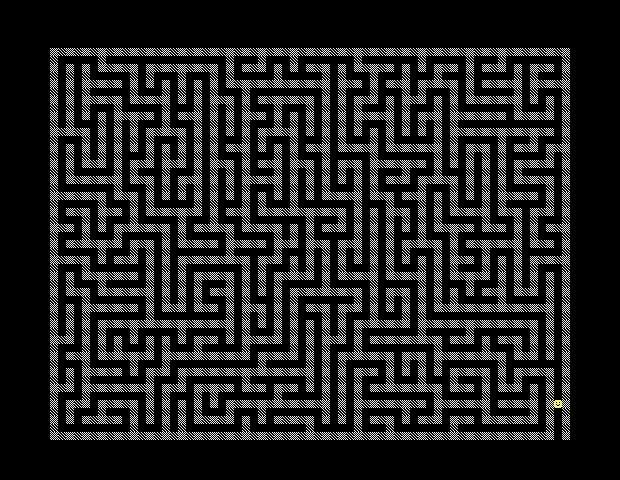
\includegraphics[width=0.75\linewidth]{maze.jpg}
		\caption{原始迷宫图像}
	\end{figure}
	
	
	
	将解析后的迷宫表示为确定性 GridWorld：
	\begin{itemize}
		\item 状态 $s=(r,c)$ 为一个可通行栅格；
		\item 动作为 $A=\{\mathrm{U},\mathrm{D},\mathrm{L},\mathrm{R}\}$；
		\item 若相邻栅格可通行，则转移到该栅格，否则该动作不作为合法动作；
		\item 终点 $g$ 为吸收状态；
		\item 每走一步奖励为 $-1$，终点价值为 $0$。
	\end{itemize}
	
	因此，最优价值函数满足 Bellman 最优方程：
	\[
	V^*(g)=0,\qquad
	V^*(s)=\max_{a\in A(s)}\left[-1+V^*\bigl(T(s,a)\bigr)\right],
	\quad s\neq g.
	\]
	
	对应的最优动作价值函数为
	\[
	Q^*(s,a)=-1+V^*\bigl(T(s,a)\bigr),
	\qquad
	\pi^*(s)=\arg\max_{a\in A(s)}Q^*(s,a).
	\]
	
	由于每一步奖励相同且为负数，最大化累计奖励等价于最小化步数。于是
	$V^*(s)=-d(s,g)$，其中 $d(s,g)$ 是状态 $s$ 到终点 $g$ 的最短步数。程序采用
	从终点反向传播的 Bellman 更新来得到收敛后的 $V^*$ 和 $Q^*$，再从黄色起点按
	$Q^*$ 贪心选取动作，从而得到最短路径。
	
	\subsection{代码结果与结论}
	

	
	有两种给定终点的方式：直接在图像上点击目标位置，或输入终点的行列坐标后点击
	``求解''。若终点是墙体或在迷宫外，代码会提示不可通行；若可通行，则显示路径和
	最短步数。
	
	测试结果如下：
	
	\begin{center}
		\begin{tabular}{lll}
			\toprule
			终点 & 结果 & 最短步数 \\
			\midrule
			$(25,33)$ & 可到达，自动示例终点 & $619$ \\
			$(1,1)$ & 可到达 & $343$ \\
			$(10,10)$ & 位于墙体或不可通行区域 & -- \\
			\bottomrule
		\end{tabular}
	\end{center}
	
	自动示例会选择从起点出发距离最远的可通行终点。实验中，起点为 $(44,63)$，自动终点为 $(25,33)$，
	最短路径长度为 $619$ 步，路径共包含 $620$ 个栅格状态。
	
	\begin{figure}[h]
		\centering
		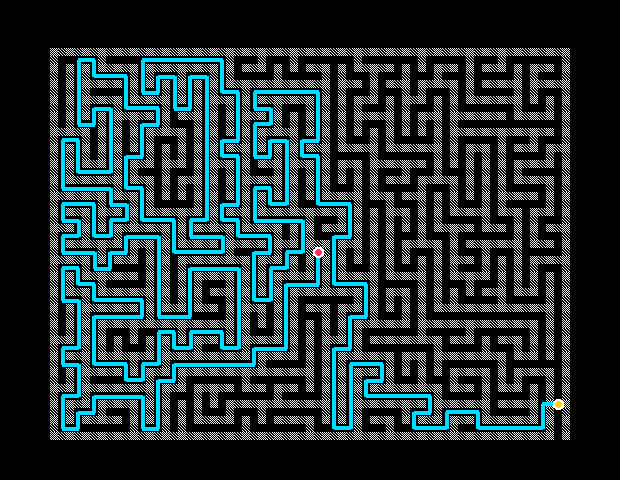
\includegraphics[width=0.75\linewidth]{demo_path.png}
		\caption{自动示例终点 $(25,33)$ 的最短路径}
	\end{figure}
	

	该方法将图像迷宫转化为有限状态 MDP，并通过 Bellman 最优方程计算最优
	$Q$ 值。由于奖励设计为每步 $-1$，所得最优策略天然对应最短路径；若给出的终点
	不是可通行状态，程序会直接判断为不能到达。交互式界面可以直观展示不同终点对应的
	路径规划结果。
	
\end{document}
